
\paragraph{User Module Sub-system}
\subparagraph{Class Diagram}
The class diagram of the user sub-system makes use of the template method so that if need be one can easily construct different types of users with minimal code modifications.

\begin{figure}[H]
	\centering
	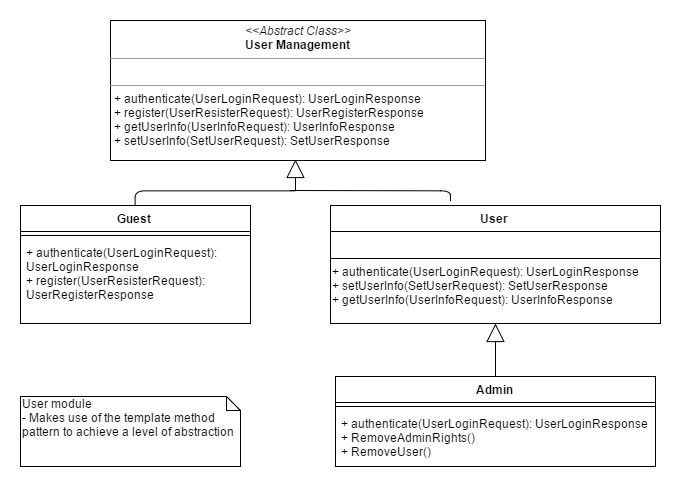
\includegraphics[width=\textwidth]{img/UserClassDiagram.jpg}
	\caption{User Class Diagram}
\end{figure}



\subparagraph{Deployment Diagram}

\begin{figure}[H]
%	\centering
%	\includegraphics[width=\textwidth]{img/}
%	\caption{}
\end{figure}


\subparagraph{Activity Diagram}

\begin{figure}[H]
	%	\centering
	%	\includegraphics[width=\textwidth]{img/}
	%	\caption{}
\end{figure}


\subparagraph{Sequence Diagram}

\begin{figure}[H]
		\centering
		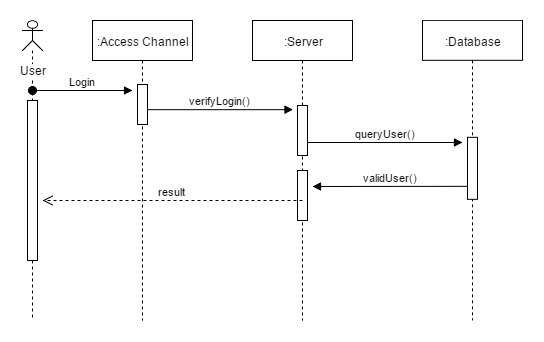
\includegraphics[width=\textwidth]{img/UserSequence.jpg}
		\caption{User Login}
\end{figure}



\subparagraph{State Diagram}

\begin{figure}[H]
	%	\centering
	%	\includegraphics[width=\textwidth]{img/}
	%	\caption{}
\end{figure}




\subparagraph{Use Case Diagram}

\begin{figure}[H]
		\centering
		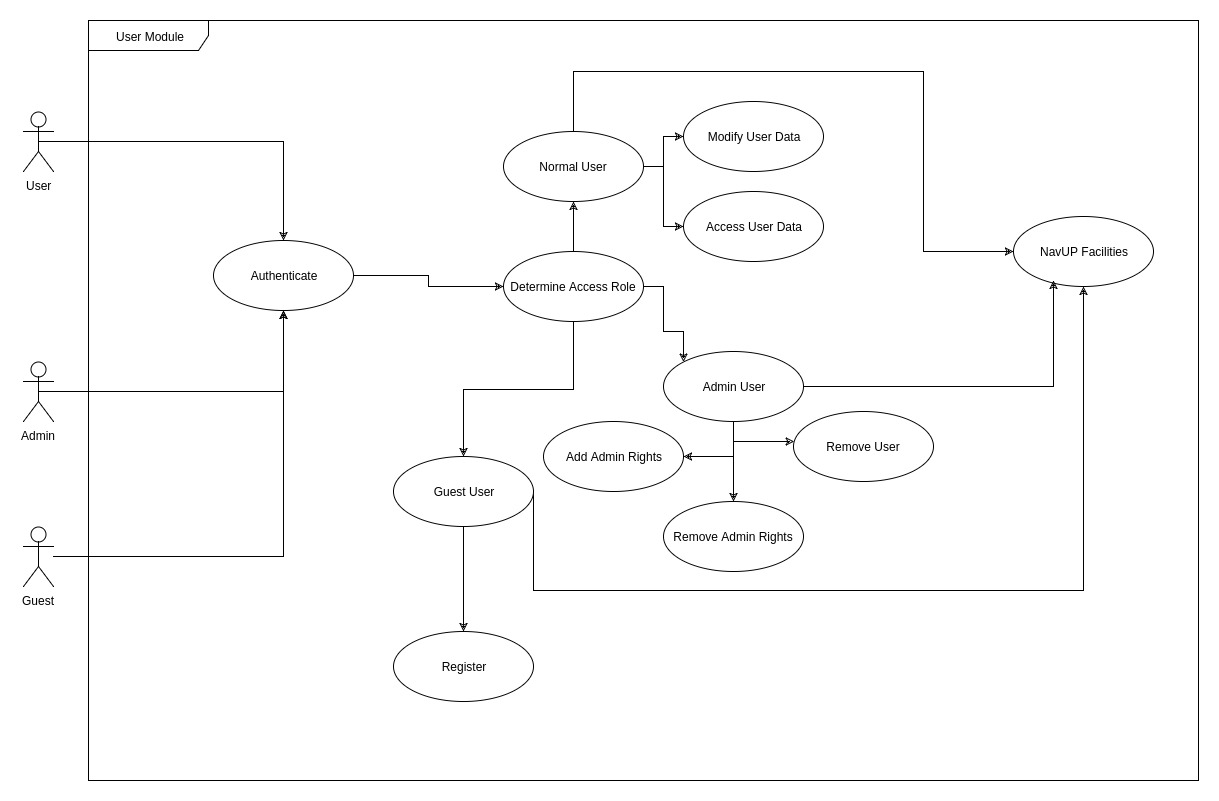
\includegraphics[width=\textwidth]{img/UserUseCase.jpg}
		\caption{User Login with core functionality }
\end{figure}



